\section{Influenza-like-Illness Forecasting}
In this section we analyze the forecasts generated for Influenza-like-Illness
or ILI events. For ILI, we concentrated on short-term forecasts for the first
2 years of \EMBERS. We shifted our focus to long-term forecasts for the subsequent
years. We analyze both types of forecast here for general performance and
analyze in details a few successful forecasts which showcased the strength
our system. There were a number of \EMBERS~ILI forecasts which significantly
deviated from the target sources. We analyzed these scenarios and discuss in
details some of the weakness of \EMBERS. These scenarios also helped us to
increase the robustness of our system.

% \prithwi{TODO:}
% \begin{itemize}
  % \item Histogram of short-term forecasts QS/lead time
  % \item Histogram of long-term forecasts QS/lead time
  % \item CI for all categories. -- signficance of bad/good forecasts.
% \end{itemize}

\subsection{Successes}
% \prithwi{Long-term and short term}
Our models for ILI were tuned over time to incorporate our findings over time.
Over the course of our project we sent a number of perfect warnings (QS$=4.0$)
as well as significant number of high quality warnings ( QS $\geq 3.0$). For
example, we sent several ILI case count warnings for Chile for event date
08/07/2013. The actual value for the said date was 626 while we sent a first
warning for 581 (QS: $3.71$) and a second update (QS: $3.95$).
Figure~\ref{fig:ili_temporal} shows a temporal history of high quality warnings.
As can be seen, the number of perfect warnings sent increased over time without
sacrificing the number of high quality warnings significantly.

We also show a distribution of the sent warnings, by combining updates for
each event date, in figure~\ref{fig:ili_hist}. As can be seen, we can see a
dual peak distribution with the first peak around the mean score and the second
one around the perfect score of $4.0$.


\begin{figure}
  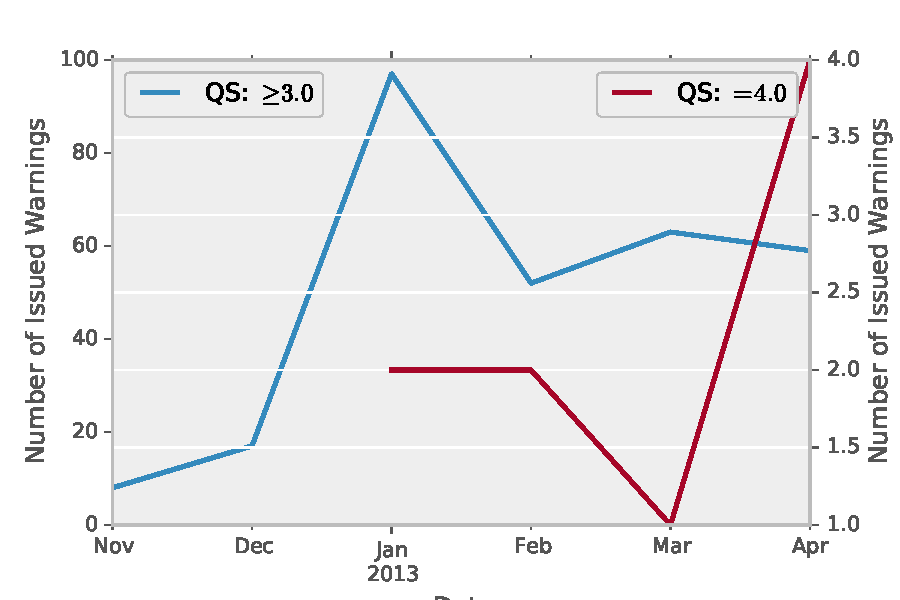
\includegraphics[width=0.4\textwidth]{../figures/ili/HighQualityWarnings.pdf}
  \caption{\label{fig:ili_temporal}Number of High quality ILI warnings over time.}
\end{figure}

\begin{figure}
  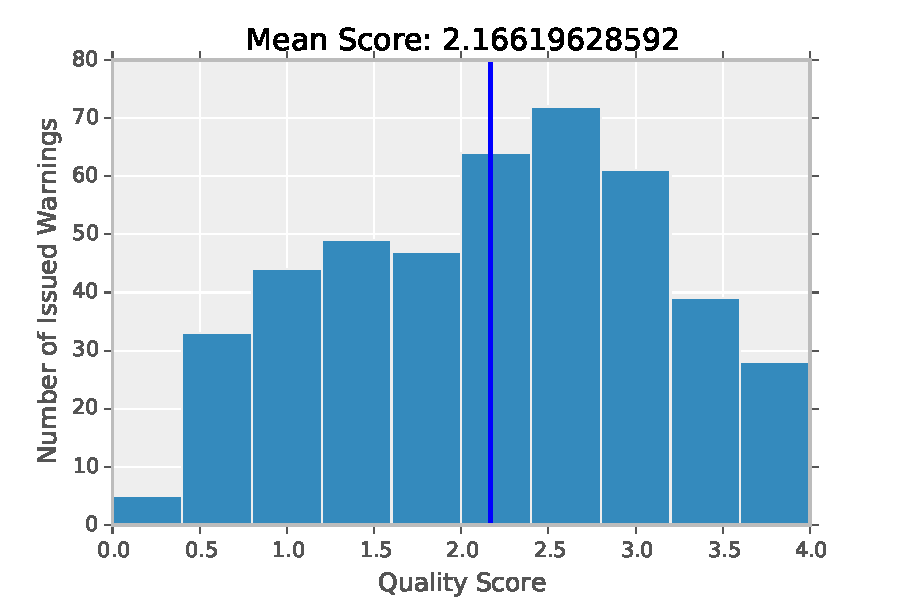
\includegraphics[width=0.4\textwidth]{../figures/ili/CombinedAllScore.pdf}
  \caption{\label{fig:ili_hist_all}Histogram of Quality scores for ILI warnings
  combining updates for each event date.}
\end{figure}

% \begin{figure*}[tb!]
  % \subcaptionbox{}{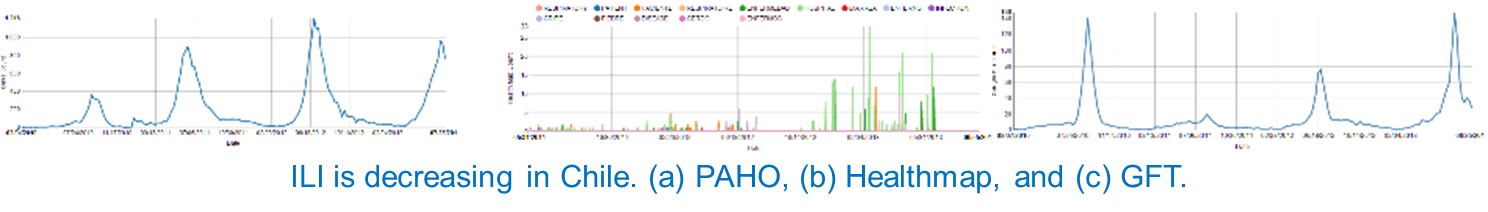
\includegraphics[width=0.9\textwidth]{../figures/ili/narrative1.png}}
  % \\
  % \subcaptionbox{}{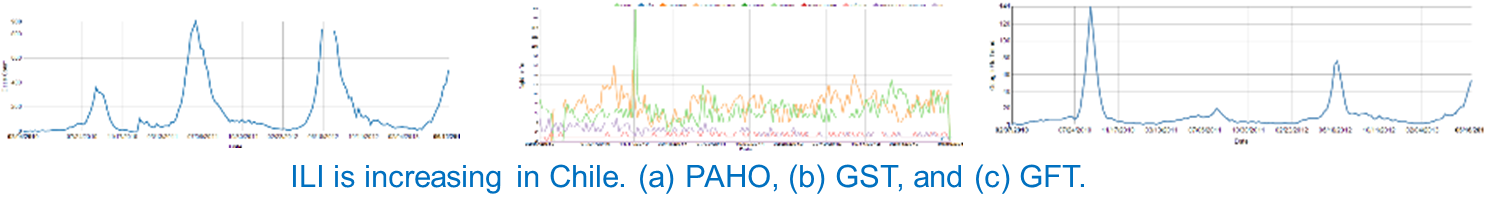
\includegraphics[width=0.9\textwidth]{../figures/ili/narrative3.png}}

  % \caption{\label{} ILI short-term: success stories}
% \end{figure*}

During the course of the project we were allowed to update our warnings, if
needed, before the event is published. Figure~\ref{fig:ili_hist_all} showed
the distribution of scores for warnings by taking the mean scores
of all the updates issued.
We further analysed our update scheme in Figure~\ref{fig:ili_hist:compare}.
As can be seen we see a significant upward shift in our score from first
update to last update. We can also see that if the best update could have
been predicted our scores would have been higher.

\begin{figure*}[tb!]
  \subcaptionbox{}{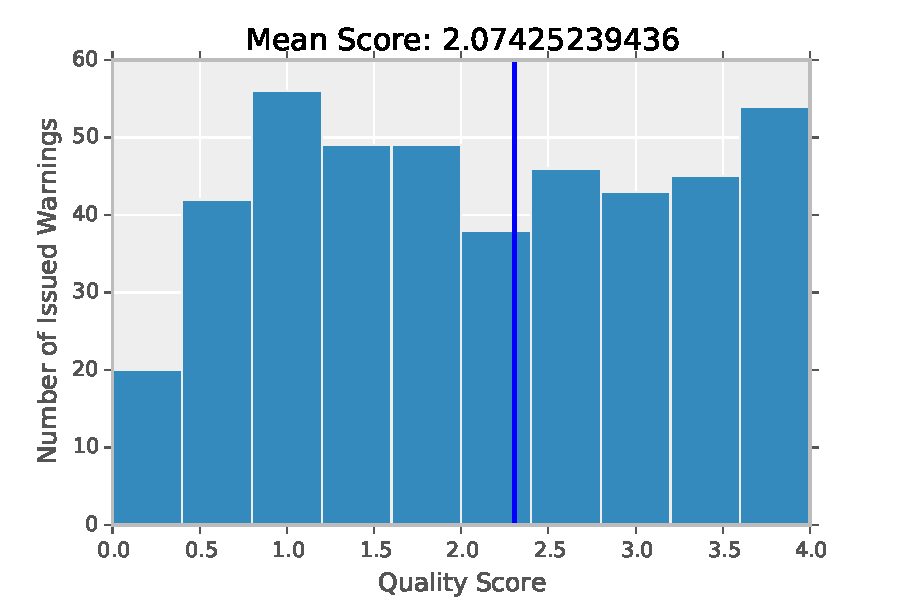
\includegraphics[width=0.30\textwidth]{../figures/ili/CombinedFirstScore.pdf}}

  \subcaptionbox{}{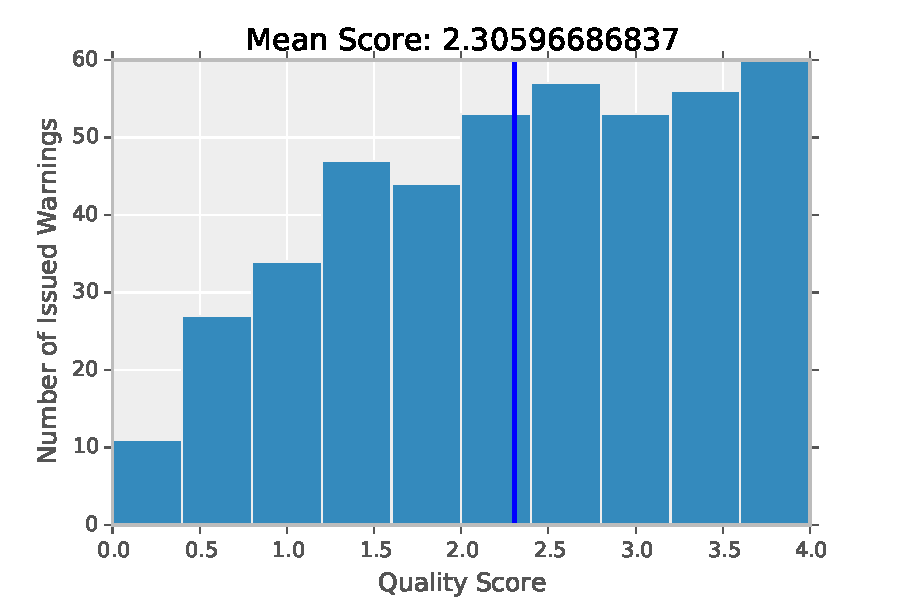
\includegraphics[width=0.30\textwidth]{../figures/ili/CombinedLastScore.pdf}}

  \subcaptionbox{}{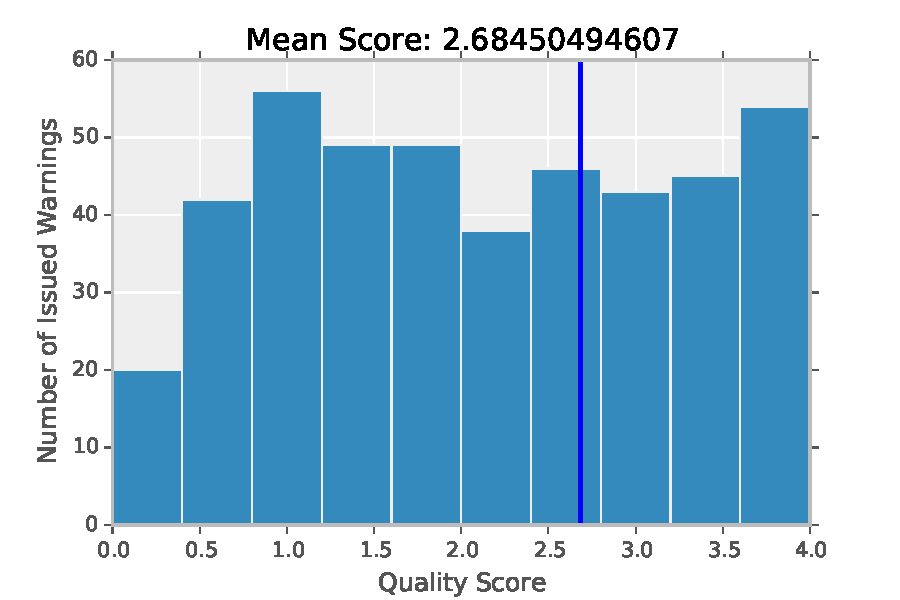
\includegraphics[width=0.30\textwidth]{../figures/ili/CombinedBestScore.pdf}}

  \caption{\label{ref:ili_hist:compare} Histogram of Quality Scores for ILI warnings
  for each event date. (a) Considering the first update, (b) Considering the last update,
  and (c) Considering the best update.}
\end{figure*}

% \begin{itemize}
  % \item {\bf Short-term:} ILI case counts for Chile for event date 08/07/13.
    % \begin{itemize}
      % \item Actual value: 626
      % \item First update: 581 (QS: 3.71)
      % \item Second update: 619 (QS: 3.95)
      % \item Possible reason: season occuring around same time, similar shape.
    % \end{itemize}

  % \item {\bf Long-term:} ILI seasonal predictions for Bolivia
    % \begin{itemize}
      % \item Total flu/SRV count
      % \item Peak date for flu/SRV
    % \end{itemize}
% \end{itemize}

For our long term forecasts, we were able to send perfect predictions for a
number of countries such as Bolivia for a number of event types such as
peak date for flu/SRV and Total Flu count.

\subsection{failures}

We also analysed our performance for significant low scores.
Figure~\ref{fig:ili_hist:arg} shows the distribution of scores for Argentina where
we performed poorly with respect to to other countries such as Bolivia. As can be seen the
distribution is unimodal around the mean. The lack of our perfect warnings
could be attributed to more unstable nature of ILI surveillance in the country as
well as the physical size of the country where a single surveillance
center may be composed of trends from several disparate regions.

\begin{figure}
  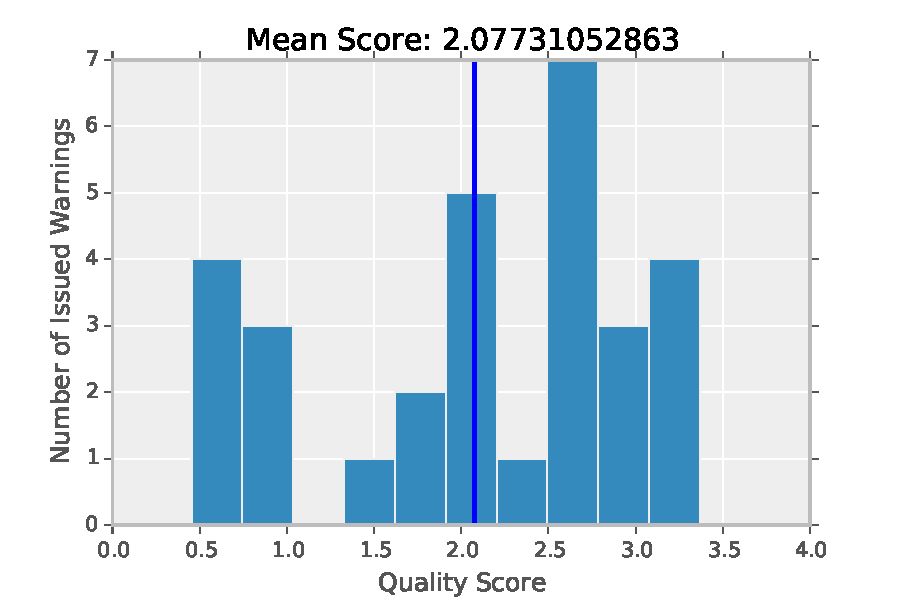
\includegraphics[width=0.4\textwidth]{../figures/ili/Failure_Argentina.pdf}
  \caption{\label{fig:ili_hist:arg}Histogram of Quality scores for ILI warnings
  for Argentina.}
\end{figure}

% \begin{itemize}
  % \item {\bf Short-term:} ILI case counts for Argentina
    % \begin{itemize}
      % \item Seasonality?
    % \end{itemize}
  % \item {\bf Long-term:} ILI seaonal predictions for Mexico
    % \begin{itemize}
      % \item Shifts in seasons.
    % \end{itemize}
% \end{itemize}

